\documentclass[10pt]{article}
\usepackage[margin=.6in]{geometry}
\usepackage{amssymb}
\usepackage{amsmath}
\usepackage{amsthm}
\usepackage{multirow}
\usepackage{graphicx}
\usepackage{caption}
\usepackage{subcaption}

\begin{document}
\def\R{\mathbb{R}}

\begin{center}
    \textbf{MATH 495 - Capstone \\
    Exit Exam by Tim Sizemore \\
    Monday, February 3, 2014}
\end{center}

[5 points] \textbf{Name:\line(1,0){147}}
\\
\begin{enumerate}
    \item \verb![12 points]!Use the function $g(x)$ defined below to answer the following questions: \\
    $$
    g(x) =
    \begin{cases}
        x + 5 & \text{for } x < 0  \\
        x^2 + 1 & \text{for } 0 \le x \le 2 \\
        3 & \text{for } x > 2
    \end{cases}
    $$

    \begin{enumerate}
        \item $\displaystyle\lim_{x \to 0^-} g(x) = \lim_{x \to 0^-} x + 5 = 5$
        \item $\displaystyle\lim_{x \to 0^+} g(x) = \lim_{x \to 0^+} x^2 + 1 = 1$
        \item $\displaystyle\lim_{x \to 0} g(x) \text{does not exist}$
        \item $\displaystyle\lim_{x \to \infty} g(x) = \lim_{x \to \infty} 3 = 3$
    \end{enumerate}

    \item \verb![16 points]!\textbf{Possums and Leslie Matrices} \\
    The following table lists reproduction and survival rates for the female population of possum in the United States.
    Suppose possums give birth only once a year, which dictates a natural time step of one year. Due to natural life
    span and trac possums seldom if ever live longer than 5 years, which gives a natural stopping point for the age
    classes.

        \begin{center}
            \textbf{Birth and Survival Rates for Female Possums} \\
            \vspace{4mm}
            \begin{tabular}{|c|c|c|}
                \hline
                Age (years) & Birth Rate & Survival Rate \\
                \hline
                0 - 1 & 0.0 & 0.6 \\
                1 - 2 & 1.3 & 0.8 \\
                2 - 3 & 1.8 & 0.8 \\
                3 - 4 & 0.9 & 0.4 \\
                4 - 5 & 0.2 & 0.0 \\
                \hline
            \end{tabular}
        \end{center}

    Let $x_1$ represent the number of possums in the 0-1 year age group; $x_2$ the number of possums in the 1-2 year age
    group; $x_3$ the number of possums in the 2 - 3 year age group; $x_4$ the number of possums in the 3 - 4 year age group;
    and $x_5$ be the number of possums in the 4 - 5 year age group. \\
    Calculate the rate at which the population is changing over each of those years by filling in the table below. Round
    your answers to THREE DECIMAL PLACES.

    \begin{tabular}{|c|p{2cm}|p{2cm}|c|p{2.2cm}|p{2.2cm}|p{2.2cm}|}
        \cline{2-7}
        \multicolumn{1}{c|}{} & Between Years 0 \& 1 & Between Years 1 \& 2 & & Between Years 11 \& 12 & Between Years 12 \& 13 & Between Years 13 \& 14 \\
        \hline
        & & & & & & \\
        $\displaystyle k = \frac{\text{Pop. at Year} n + 1}{\text{Pop. at Year} n}$ & & & & & & \\
        & & & & & & \\
        \hline
        & & & & & & \\
        Total Change: $k-1$ & & & & & & \\
        & & & & & & \\
        \hline
    \end{tabular}

\newpage

\item \verb![16 points]!The temperature at a point $(x, y$) on a metal plate is $T(x, y) = 4x^2 + 4xy +y^2$. An ant on the plate walks
    around the circle of radius 5 centered at the origin. Where are the highest and lowest temperatures encountered by
    the ant? Use the Lagrange Multiplier Method to the maximum and minimum of $T(x, y)$ subject to the equation
    given by the ant's path.
    \begin{eqnarray*}
        \nabla T(x,y)
        & = & \lambda \nabla g(x,y) \\
        \langle 8x + 4y,4x + 2y \rangle
        & = & \lambda \langle 2x,2y \rangle
    \end{eqnarray*}
    So our system of equations is
    \begin{eqnarray}
        8x + 4y
        & = & \lambda(2x)\label{1} \\
        4x + 2y
        & = & \lambda(2y)\label{2} \\
        x^2 + y^2
        & = & 25\label{3}
    \end{eqnarray}
    Mulitplying \ref{2} by -2 and adding to \ref{1}
    \begin{eqnarray*}
        -8x - 4y & = & -4\lambda y \\
        8x + 4y & = & 2\lambda x \\
        & \Downarrow &\\
        0 & = & 2\lambda x - 4\lambda y \\
        0 & = & 2\lambda(x - 2y) \\
        & \Downarrow & \\
        \lambda = 0 &\text{ or }& x = 2y
    \end{eqnarray*}
    If $\lambda = 0$, then
    \begin{eqnarray*}
        4x + 2y & = & 0 \\
        4x & = & -2y \\
        x & = & -\frac{1}{2}y \\
        & \Downarrow & \\
        \left(-\frac{1}{2}\right)^2 + y^2 & = & 25 \\
        \frac{1}{4}y^2 + y^2 & = & 25 \\
        \frac{5}{4}y^2 & = & 25 \\
        y^2 & = & 20 \\
        y & = & \pm\sqrt{20} \\
        y & = & \pm2\sqrt{5}
    \end{eqnarray*}
    As $x = -\frac{1}{2}y $ then $(-\sqrt{5},2\sqrt{5}),(\sqrt{5},-2\sqrt{5})$\\
    \\
    If $x = 2y$, then
    \begin{eqnarray*}
        (2y)^2 + y^2 & = & 25 \\
        5y^2 & = & 25 \\
        y^2 & = & 25 \\
        y & = & \pm\sqrt{5}
    \end{eqnarray*}
    As $x = 2y$ then $(2\sqrt{5},\sqrt{5}),(-2\sqrt{5},-\sqrt{5})$. \\
    Checking $z$-values: \\
    $(2\sqrt{5},\sqrt{5}) \rightarrow 80 + 40 + 5 = 125$ (max) \\
    $(-2\sqrt{5},-\sqrt{5}) \rightarrow 80 + 40 + 5 = 125$ (max) \\
    $(-\sqrt{5},2\sqrt{5}) \rightarrow 20 - 40 + 20 = 0$ (min) \\
    $(\sqrt{5},-2\sqrt{5}) \rightarrow 20 - 40 + 20 = 0$ (min) \\

    \newpage

\item \verb![18 points]!Let $A$ and $B$ be subsets of a universal set $U$. Prove that $\overline{A\cup B} = \overline{A}\cap \overline{B}$. \\
    \textbf{Proof:} \\
    (a) Prove $ \overline{A\cup B}\subseteq\overline{A}\cap\overline{B}$. \\
    \\
    Let $x\in\overline{A\cup B}$. \\
    Then $x\notin(A\cup B)$. \\
    So, $\neg(x\in(A\cup B))$. \\
    So, $\neg(x\in A \text{or} x\in B)$. \\
    So, distributing the negation, $x\notin A \text{ and }x\notin B$. \\
    Thus, $x\in\overline{A} \text{ and } x\in\overline{B}$. \\
    So $x\in\overline{A}\cap\overline{B}$. \\
    Since $x$ was an arbitrary element, it is true for all elements $x$, if $x\in\overline{A\cup B}$, then $x\in\overline{A}\cap\overline{B}$. Hence, $\overline{A\cup B}\subseteq\overline{A}\cap\overline{B}$. \\

    (b) Prove $\overline{A}\cap\overline{B}\subseteq\overline{A\cup B}$. \\
    \\
    Let $x\in\overline{A}\cap\overline{B}$. \\
    So $x\in\overline{A}\text{ and } x\in\overline{B}$. \\
    Thus, $x\notin A \text{ and } x\notin B$. \\
    "Factoring out" a negation, we get $\neg(x\in A \text{ or }x\in B)$. \\
    So, $\neg(x\in(A\cup B)$. \\
    Thus, $x\notin(A\cup B)$. \\
    So, $x\in\overline{A\cup B}$. \\
    Since $x$ was an arbitrary element, it is true for all elements $x$, if $x\in\overline{A}\cap\overline{B}$, then $x\in\overline{A\cup B}$. Hence, $\overline{A}\cap\overline{B}\subseteq\overline{A\cup B}$. \\
    \\
    Since $\overline{A\cup B}\subseteq\overline{A}\cap\overline{B} \text{ and } \overline{A}\cap\overline{B}\subseteq\overline{A\cup B}$, we know that $\overline{A\cup B} = \overline{A}\cap\overline{B}$. \\

\item \verb![18 points]!\textbf{Verifications} \\
    \vspace{-3mm}
    \begin{enumerate}
        \item Let $W$ be the subset of $\R^{2\text{x}2}$ given by
        \[
            W = \left\{ A\in\R^{2\text{x}2 } \; \middle| \; A = \left[
                                                \begin{array}{cc}
                                                    a & a + 2 \\ 
                                                    b & c
                                                \end{array}
                                                \right]\right\}
        \]
        Determine whether $W$ forms a subspace of $V = \R^{2\text{x}2}$ over the field $F = \R$. Show all of your work.
        \item Let
        \[
            \alpha_1 = \left[
                \begin{array}{c}
                    3 \\
                    -6
                \end{array}\right],\; \alpha_2 = \left[
                \begin{array}{c}
                    -1 \\
                    2
                \end{array}\right],\text{ and } \alpha_3 = \left[
                \begin{array}{c}
                    1 \\
                    -4
                \end{array}\right]
        \]
        Is $\alpha = \left[
                \begin{array}{c}
                    8 \\
                    -3
                \end{array}\right] \in$ \;Span($\alpha_1,\alpha_2,\alpha_3$)? Justify your answer.
        \item Identify if the linear transformation, $T$, is invertible, showing your work. Let $T : \R^3\rightarrow\R^3$ be given by
                \[
                    T\left(\left[
                        \begin{array}{c}
                            x \\
                            y \\
                            z
                        \end{array}\right]\right) = \left[
                        \begin{array}{c}
                            x + y \\
                            -y \\
                            2x
                        \end{array}\right]
                \]
    \end{enumerate}

    \newpage

\item \verb![15 points]! \textbf{Washer Method} \\
    When the area being rotated is \underline{\textbf{NOT} always flush} to the axis of rotation, we can't use the disc method because our
    cross-section has a "hole" in it, giving us a \textbf{washer} rather than a disc. Once again, the representative rectangle is
    drawn \underline{\underline{\textbf{perpendicular}}} to the axis of rotation. \\
    \textbf{Vertical Rectangles (Horizontal axis of rotation)}

    \begin{figure}[h!]
        \centering
        \begin{subfigure}[b]{0.5\textwidth}
            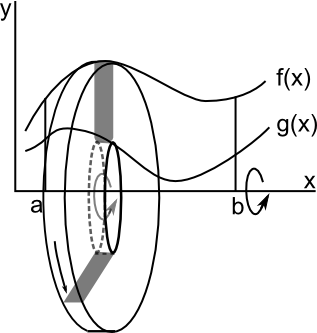
\includegraphics[scale=.75]{wvr.png}
            \caption{Using Vertical Rectangles when Rotating}
            \label{fig:wvr}
        \end{subfigure}
        \begin{subfigure}[b]{0.3\textwidth}
            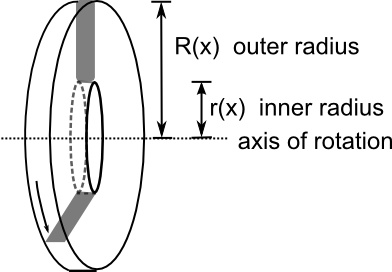
\includegraphics[scale=.60]{w.png}
            \caption{The Washer}
            \label{fig:w}
        \end{subfigure}
        \caption{Visualizing the Derivation of the Washer Method}\label{fig:washers}
    \end{figure}

    Think of the rectangle \textit{as pointing to the axis whose variable appears in the radius function}. Here we have an inner
    radius, $r(x)$, and an outer radius, $R(x)$, both functions of $x$. Thus, the volume of the washer is given by:

    \begin{align*}
        \text{Volume of washer} & = \text{(Volumer of outer disc) - (Volume of inner disc)} \\
        & = \pi(R(x))^2\Delta x - \pi(r(x))^2\Delta x
    \end{align*}

    Thus, the volume of the region created by rotating this area about the axis of rotation is:

    \[
        V = \int_a^b \pi(\underbrace{R(x)}_{\text{Outer Radius}})^2 - (\underbrace{r(x)}_{\text{Inner Radius}})^2\,dx
    \]

    Set up the equation for the volume generated by rotating the area between $y = \sqrt{x}$ and $y = 2$ and the $y$-axis about
    the $x$-axis.
    \begin{figure}[h!]
        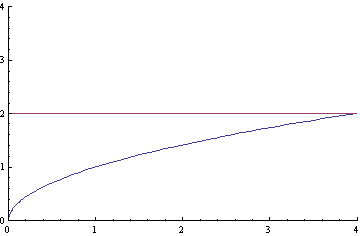
\includegraphics[scale=.35]{sxy.png}
    \end{figure}

\end{enumerate}
\end{document}
